\section{Approach}
\label{sec:approach}

The training of a dialogue summarization model is divided two stages: 
post-training and fine-tuning. The model can be any seq-to-seq PLMs
and it remains unchanged
except for the parameters which are updated stage by stage.
We will elaborate on the post-training stage in the rest of this section.
%We will focus on the post-training next. 
%In Stage 1, we construct dialogue-to-text rephrase pairs extracted from the original dialogue summarization data.
%The model then learns to rephrase from dialogue utterances into
%third-person narratives using the PGG task.
% In Stage 2, the model is fine-tuned by an auto-regressive
%text generation task as usual using the original dataset. We will elaborate on Stage 1 in the rest of this section.
%

%\begin{figure}[t]
%	\centering
%	\subfigure[Overall Approach]{
%		%		\centering
%		%		\begin{minipage}[t]{0.5\linewidth}
%		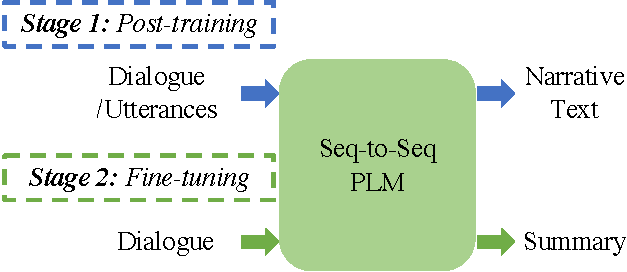
\includegraphics[scale=0.7]{stage.pdf}\label{fig:stage}
%		%		\end{minipage}
%	}
%	
%	\subfigure[PGG Task]{
%		%	\centering
%		%	\begin{minipage}[t]{0.5\linewidth}
%		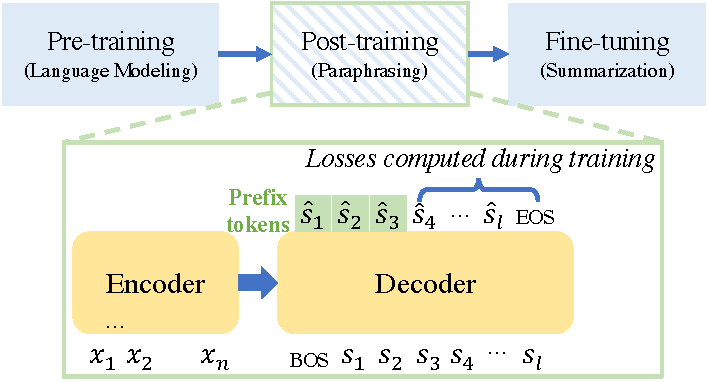
\includegraphics[scale=0.7]{pgg.pdf}\label{fig:pgg}
%		%	\end{minipage}
%	}
%	\caption{Illustrations of our overall approach and PGG task. BOS and EOS are special tokens indicating the beginning and the end of decoding.}
%	\label{fig:approach}
%\end{figure}


%\begin{figure}
%	\centering
%	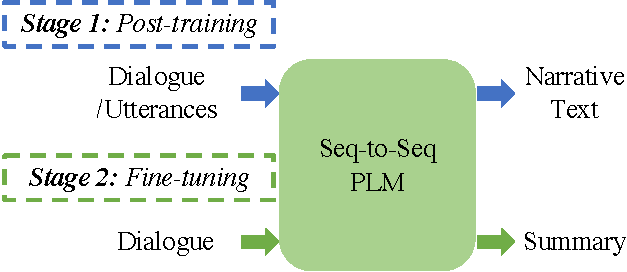
\includegraphics[width=0.8\columnwidth]{stage.pdf}
%	\caption{An illustration of our approach.}
%	\label{fig:stage}
%\end{figure}
%\subsection{Post-training for Rephrasing} 
%The intuition for post-training is to narrow down the comprehension gap between 
%dialogue and narrative text. To this end, we post-train the model to learn the rephrasing ability, 
%as a preliminary competency for dialogue summarization. We construct rephrasing datasets in different ways and propose a new prefix-guided generation task.
%

\subsection{Pseudo-paraphrase Dataset Construction}
\label{sec:rephrasedata}
%Since there is no available dialogue-to-text rephrasing data as far as we know, 
We construct rephrasing datasets from the dialogue summarization dataset 
itself.  
%In this way, we don't need additional efforts to collect or label external data. 
%One advantage is this kind of dataset is in the same domain as the final dialogue summarization, 
%doing away the need for domain adaptation in fine-tune stage.
%All of the data are transformed from the training and validation sets, leaving the test set untouched to avoid information leak.
The original dialogue summarization dataset (\textbf{DSum}) 
is made up of dialogue-summary ($D$-$S$) pairs. Each dialogue $D$
is a sequence of utterances and can be concatenated into a whole sequence: 
\begin{equation}
	D = \{U_1, U_2, ..., U_T\} = \{x_1, \ldots, x_n\}
\end{equation}
Each turn $U_t$ is in the form of [$r_t$: $u_t$], where $r$ is a speaker and 
$u$ is the actual utterance. 

Our goal is to create more dialogue to narration kind of paraphrasing pairs. The most
intuitive approach is to divide $S$ into sentences, and pair each sentence
to $D$. We call such pairs ``pseudo-paraphrases'' because the output
sentence (which we call $p$) isn't exactly the paraphrase of the whole 
input, but rather part of the input.%, as $p$ is part of the summary of $D$.

However, doing this poses two challenges: 1) $S$ is a coherent piece of 
text, and its sentences may depend on each other, so a single sentence $p$
out of it may not stand by itself; 2) one $D$ will be paired with
several different $p$, and it is hard for the model to distinguish 
the meaning of these pairs. 

\begin{table}[th]
	\scriptsize
	\centering
	\begin{tabular}{lll}
		\toprule[1pt]
		\textbf{Datasets} & \textbf{Input} & \textbf{Output} \\
		\midrule[1pt]
%		{DialIndirect} & $U_{1\sim8}$& \makecell[l]{Katarina says,``Hello, I got ...\\ we work together'' Jill says,\\``Hi :) ......  nice and sunny''}\\
%		\midrule[1pt]
%		{ExtSum} &$U_3$, $U_6$ & \makecell[l]{Katarina ...... a flat from Liz.\\ She will ...... after 6 pm.} \\
%		\midrule[1pt]
%		{ExtSumM} &$U_{3\sim6}$&\makecell[l]{Katarina ...... a flat from Liz.\\ She will ...... after 6 pm.}  \\
%		\midrule[1pt]
%		\multirow{2}{1cm}{{ExtSent/\\ExtSentM}}&$U_3$&Katarina ...... a flat from Liz. \\
%		\cmidrule{2-3}
%		& $U_6$ &Katarina will ...... after 6 pm. \\
%		\midrule[1pt]
		{DSum} & $U_{1\sim8}$& \makecell[l]{Katarina wants to rent a flat from Liz.\\ She will come visit it today after 6 pm.}\\
		
		\midrule[1pt]
		\multirow{2}{1cm}{{DialSent}} & $U_{1\sim8}$ &\textit{\underline{Katarina} wants} to rent a flat from Liz. \\
		\cmidrule{2-3}
		&$U_{1\sim8}$ &\textit{\underline{Katarina} will come} visit it today after 6 pm. \\
		
		\bottomrule[1pt]
	\end{tabular}
	\caption{Example pseudo-paraphrase pairs generated from the example in Figure~\ref{fig:example}. One pair in DSum becomes two pairs in DialSent. The prefix tokens determined by linguistic features, NOUN and ROOT, are underlined and italic respectively.}
%ExtSent and ExtSentM get the same training pairs in this case.
\label{tab:datasets}
\end{table}

To solve 1) we apply coreference resolution\footnote{We use \url{https://spacy.io/}.} on $S$ and convert every pronoun in it to the full reference 
first, before splitting the summary $S$ into sentences. 
Sentence with fewer than 3 words (e.g., ``Ally agree'') 
are discarded since it carries too little information.  
The set of data pairs thus created is called (\textbf{DialSent}). 
An example is in 
\tabref{tab:datasets}.

To tackle 2), one obvious thought is to further split $D$ into sets of sentences
in which each set corresponds to a sentence $p$ in the summary.
However, our extensive experiments (see \apxref{sec:para}) showed that none of the 
straight-forward heuristics work well to establish such alignments.
This is mainly due to the fact that dialogue utterances are highly dependent. Thus, splitting operations are not optimal.
Instead of changing $D$, we decide to use the pseudo-paraphrases
directly but introduce a prefix-guided generation task to guide the model
learning to extract relevant information from $D$.
%$X=\{x_1, x_2, ..., x_n\}$ as the input to the model. The corresponding summary $Y=\{y_1, y_2, ..., y_m\}$ consists 
%of multiple sentences. $n$ and $m$ denote the number of tokens respectively.

%To make the input and output carry the same amount of information, 
%one way is to fix $D$ as input and convert utterances into indirect speech 
%as the output. \citet{ganesh2019restructuring} restructured dialogue into text with complicated rules
%%considering discourse relations among utterances for zero-shot scenarios. However, their complicated rules 
%which are not released and difficult to transfer among datasets under different scenarios. Thus, we only use simple rules to convert all of the utterances into [$r_t$ says,``$u_t$''] and concatenated as the output. We call this dataset as \textbf{DialIndirect}.
%
%Another way is fixing $Y$ as output and removing the redundant utterances in $D$ to get the rephrasing input. We take advantage of the idea of oracle extraction for news summarization~\cite{zhou-etal-2018-neural-document} and regard the combination of dialogue utterances with the highest Rouge scores computed with $Y$ as the input. Considering that utterances are highly dependent, we modify the original extraction algorithm by extracting all of the utterances lying between the extracted ones, different from the window-sized snippet selection in~\cite{liu-etal-2021-topic-aware}.  Datasets with or without this modification are called \textbf{ExtSum} and \textbf{ExtSumM} respectively.
%
%A summary $Y$ is divided into sentences to construct more rephrase pairs. 
%We use Spacy~\footnote{\url{https://spacy.io/}} to 
%%Similar extraction operations can be done between $D$ and $S$, and we get \textbf{ExtSent} and \textbf{ExtSentM} datasets.
%An example of the paraphrase pair generated from the dialogue-summary pair in Figure~\ref{fig:example} is shown 
%in Table~\ref{tab:datasets}.

\subsection{Prefix-guided Generation Task}
\label{sec:pgg}
%Although the above extraction algorithm can \KZ{What do you mean by balancing information: balance the amount of information 
%between $D$ and $Y$ or $S$}, the coreference link within $D$ will be broken caused by such hard and explicit extraction. \KZ{I don't get why the coreference links within $D$ would be a problem, since $D$ is never broken into pieces!} 
%Since the coreference resolution tools for dialogues are not nearly as good as narrative texts as 
%mentioned in~\citet{liu2021coreference}, we do not apply it on dialogues. 
%
%Instead, we propose a prefix-guided generation task for data with \KZ{unbalanced information volume}, 
Summarization for dialogues focuses on analyzing ``who-did-what'' storylines~\cite{chen2021structure} and the beginning of each summary sentence are usually different speakers or the same speaker doing different things. As a result,  using the prefix made up of ``who'' or ``who-did'' can help to select the related information from dialogues or plan the content to be generated.

In other words, we take the inspiration from content 
planning~\cite{narayan2021planning,wu-etal-2021-controllable}. 
%which assign a sequence of keywords to the decoder for controllable summaries during inference time.
When training, the first few tokens of $p$ are provided as prefix to 
the decoder. This prefix serves as an information selection hint to 
the model so it is easier to learn why that particular $p$ should be 
generated. 
%The model keeps on the generation process to complete the sentence in a third-person point of view and 
The losses are calculated between the generated tokens and reference 
tokens after the prefix as shown in Figure~\ref{fig:pgg}. 
%We determine the number of prefix tokens as the number of tokens from the beginning to the first noun or the first verb in $S$ or $Y$.
%, according to the POS tags or dependency parsing tags recognized by Spacy.
\begin{figure}[th]
	\centering
	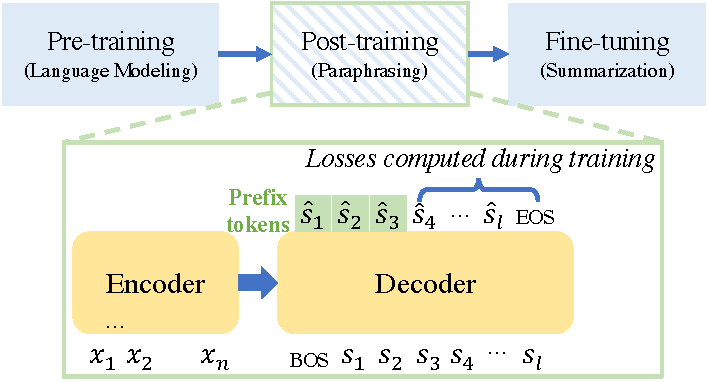
\includegraphics[width=0.75\columnwidth]{pgg.pdf}
	\caption{A illustration of our approach. 
		%The prefix is $\{\hat{s_1}, \ldots, \hat{s_3}\}$. 
BOS and EOS stand for begin and end of the sequence.}
	\label{fig:pgg}
\end{figure}

%The sequence-to-sequence model is made up of a bidirectional transformer encoder and an auto-regressive transformer decoder. The encoder takes the token sequence of $D$ as input and maps it into distributed representations $H^d$. The decoder takes $H^d$ as input and factorizes the probability of $S$ into the product of the conditional probability of each token. 
Let $p=\{s_1, \ldots, s_l\}$. 
Our prefix-guided training task is a vanilla auto-regressive generation
task minimizing the negative log-likelihood of $p$:
\begin{equation}
	\begin{aligned}
		L &= -\frac{1}{l-a}\sum_{t=a}^{l}\log P(s_t|s_{<t},H^d) \\
		%i &\sim U(a,b)
	\end{aligned}
\end{equation}
where $a$ is the number of prefix tokens. $H^d$ is the output hidden vectors of the encoder with input $D$.

%During inference, the first $b$ tokens are provided for the decoder. 
%We map the hidden states into a vocabulary distribution at each decoding step:
%%\KZ{Is it common to refer to the decoding function as $Dec$? Function names shouldn't be
%%capitalized?}
%%\begin{align}
%%P(\hat{s}_t|s, \hat{s}, b, t, H^d)= &\softmax(W_v{\rm Dec}(s_1,\ldots, s_b,\notag \\
%%&\hat{s}_{b+1},\ldots,\hat{s}_{t-1}, H^d))
%%&P(\hat{s}_t|s_{\leq b}, \hat{s}_{>b,<t},H^d)=\\
%%&\softmax(W_v{\rm Dec}(s_1,\ldots, s_b, \hat{s}_{b+1},\ldots,\hat{s}_{t-1}, H^d))
%%\end{align}
%
%\begin{align}
%		&P(\hat{s}_t|s_{\leq b}, \hat{s}_{>b,<t},H^d) =\\
%		& \softmax(W_v{\rm Dec}(s_1,..., s_b,\hat{s}_{b+1},...,\hat{s}_{t-1}, H^d))\notag
%\end{align}
%%i.e. $t>k$ in Equation \ref{eq:decoder}.
%where $Dec(\cdot)$ represents the decoder which starts decoding at 
%the $b$+$1$-th token. 

There are various ways to determine the prefix length $a$. We can take
a fixed length, a random length or a prefix up to a certain linguistic feature
such as NOUN, VERB or ROOT. 
The exact linguistic feature to use is a dataset-dependent hyper-parameter and 
can be tuned by the validation set. Examples of prefix tokens is marked in Table \ref{tab:datasets}.
%Hence $a$ is different for different training sample.
%the firWe use POS tags (``PROPN''\&``NOUN'' or ``VERB'') or dependency parsing tags (``nsubj''\&``nsubjpass'' or ``ROOT'') 
%by SpaCy to locate the noun or verb in \KZ{$S$ or $Y$} and \KZ{designate $a$ sample by sample} during training. 
%At inference time, because no ground truth of $S$ or $Y$ is given, 
%we simply set $b$ as a constant value 4.
%$k$ can be either equal to $a$ or simply set to a constant.
%$a$, $b$ and $k$ are hyper-parameters assigned as $\{2,4,3\}$ respectively.
%In a word, the post-training stage is done by the vanilla auto-regressive 
%generation task with the PGG task with DialSent or DSum.


%\subsection{Fine-tuning for Dialogue Summarization}
%
%The post-trained model can be further directly finetuned on dialogue summarization datasets to learn content selection abilities and generate a coherent summary.
%%under different scenarios and granularities.% depending on datasets. 
%%The dialogue and corresponding summary are represented as $X =\{x_1, x_2, ..., x_p\}$ and $Y=\{y_1, y_2, ..., y_q\}$, where $p$ and $q$ denote the number of tokens in the dialogue and summary. 
%We adopt the vanilla auto-regressive generation task with original dialogue-summary pairs.
%and the loss function as follow:
%\begin{equation}
%	\begin{aligned}
%		&h_1, h_2, ..., h_p = Enc(x_1, x_2, ..., x_p)\\
%		P(y_t|y_{<t},&H) = Softmax(W_vDec(y_1, ..., y_{t-1}, H))\\
%		&L = -\frac{1}{q}\sum_{t=1}^{q}\log P(y_t|y_{<t},H)
%	\end{aligned}
%\end{equation}
%where $H=\{h_1, h_2, ..., h_p\}$ represents the hidden states generated by the transformer encoder $Enc(\cdot)$.

